\begin{flushright} {\tiny {\color{gray} mms\_annulus.tex}} \end{flushright}
%~~~~~~~~~~~~~~~~~~~~~~~~~~~~~~~~~~~~~~~~~~~~~~~~~~~~~~~~~~~~~~~~~~~~~~~~~~~~~~~~~~~~~~~~~~~~~~~~~~

The domain is a hollow cylinder or inner radius $R_{i}$ and outside radius $R_{o}=1$.
Boundary conditions are prescribed both on the inside and the outside with 
${\vec \upnu}=(u,v)=(-y,x)$, or in 
polar coordinates ${\vec \upnu}=r {\vec e}_\theta$.

The gravity is radial and is set to
\[
g_x=-x/r  \quad\quad g_z=-y/r
\]
where $r=\sqrt{x^2+z^2}$, which in polar coordinates is ${\vec g}=-{\vec e}_r$.
The viscosity is also set to 1, and the density is given by
\[
\rho(r)=r^n
\]
where $n$ is a positive or nul integer. The pressure is set to zero at the outer boundary.

The gradient operator in polar coordinates writes:
\[
{\vec \nabla} = \frac{\partial }{\partial r} {\vec e}_r 
+ \frac{1}{r} \frac{\partial }{\partial \theta} {\vec e}_\theta 
\]
and the Laplacian operator:
\[
\Delta = \frac{\partial^2}{\partial r^2} + \frac{1}{r} \frac{\partial }{\partial r} + \frac{1}{r^2} \frac{\partial^2 }{\partial \theta^2}
\]
Note that in our case we need to take the Laplacian of a vector, and unfortunately the Laplacian of a vector is not the Laplacian 
of the vector's coordinates in polar coordinates (unlike cartesian coordinates). 
The Laplacian of a vector is given by\footnote{\url{https://en.wikipedia.org/wiki/Vector\_Laplacian}} 
\[
\nabla^2 \vec{A} = \nabla(\nabla\cdot\vec{A}) - \nabla\times(\nabla \times\vec{A})
=
\left(
\begin{array}{l}
\frac{\partial^2 A_r}{\partial r^2} + \frac{1}{r} \frac{\partial A_r}{\partial r} - \frac{1}{r^2} A_r  + \frac{1}{r^2} \frac{\partial^2 A_r}{\partial \theta^2}  - \frac{2}{r^2} \frac{\partial A_\theta}{\partial \theta} \\ \\
\frac{\partial^2 A_\theta}{\partial r^2} + \frac{1}{r} \frac{\partial A_\theta}{\partial r} - \frac{1}{r^2} A_\theta  + \frac{1}{r^2} \frac{\partial^2 A_\theta}{\partial \theta^2}  + \frac{2}{r^2} \frac{\partial A_r}{\partial \theta} 
\end{array}
\right)
=
\left(
\begin{array}{l}
\Delta A_r \\ \\ \Delta A_\theta
\end{array}
\right)
\]
The Stokes equation writes:
\[
-\vec\nabla p + \eta \Delta {\vec \upnu} + \rho {\vec g} = {\vec 0}
\]
The velocity solution is expected to be ${\vec \upnu}= r {\vec e}_\theta $.
The Stokes equation in polar coordinates then writes:
\[
-\frac{\partial p}{\partial r} + \Delta v_r + \rho(r) (- 1)  = 0 
\]
\[
-\frac{1}{r}\frac{\partial p}{\partial \theta} + \Delta v_\theta = 0
\]
Since $\Delta v_\theta = 0$, then $\frac{\partial p}{\partial \theta}=0$ and then the pressure is independent of $\theta$, 
which is what we expect since the density distribution is radial. 
We then focus on the first equation, and since $v_r=0$, we then obtain:
\[
\frac{\partial p}{\partial r}  = - \rho(r)
\]

\begin{itemize}
\item If $\rho(r)=1$, then 
\[
\frac{\partial p}{\partial r}  = - 1
\]
yields $p(r)=-r+C$ where C is a constant determined by means of b.c. ($p(r=1)=0$) so finally
\[
\boxed{
p(r)=1-r
}
\]

\item If $\rho(r)=r$, then 
\[
\frac{\partial p}{\partial r}  = - r
\]
so that $p(r)=-\frac{1}{2}r^2 + C$ and likewise
\[
\boxed{
p(r)=\frac{1}{2} (1- r^2)
}
\]
\end{itemize}
  
In general, by taking $\rho(r)=r^n$ with $n=0,1,...$ one arrives to a pressure field given by 
\[
\boxed{
p(r)=\frac{1}{n+1} (1- r^{n+1})
}
\]

\begin{center}
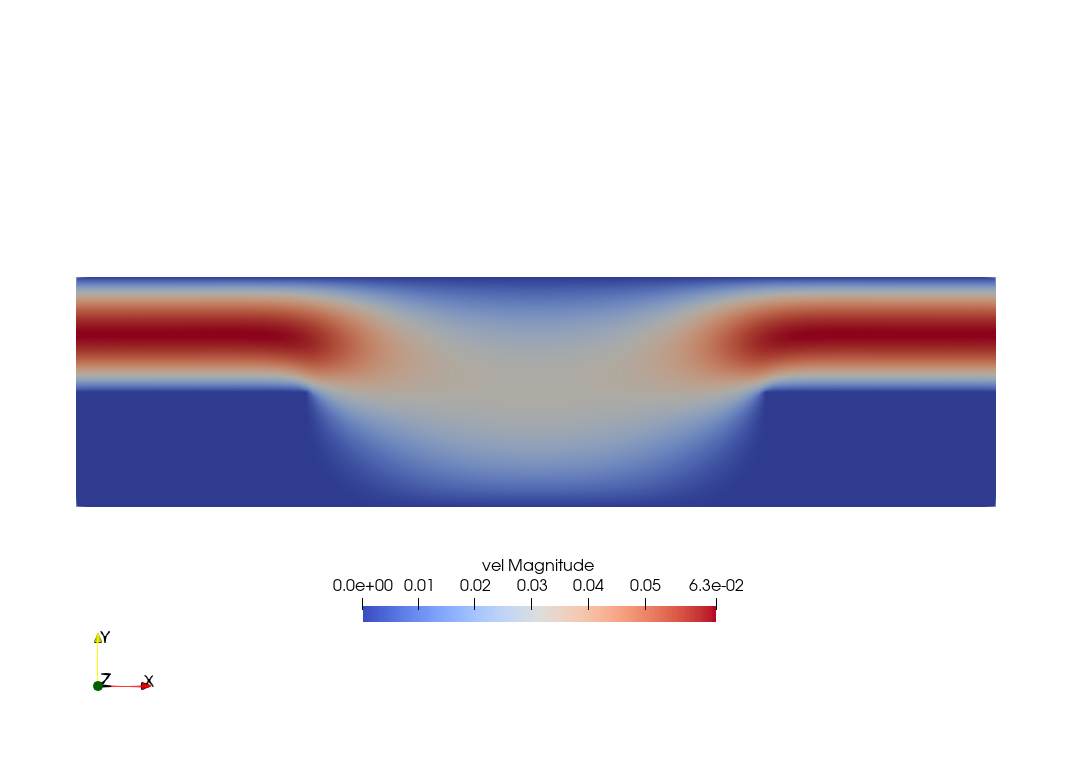
\includegraphics[width=6cm]{images/benchmark_annulus_mms/vel}
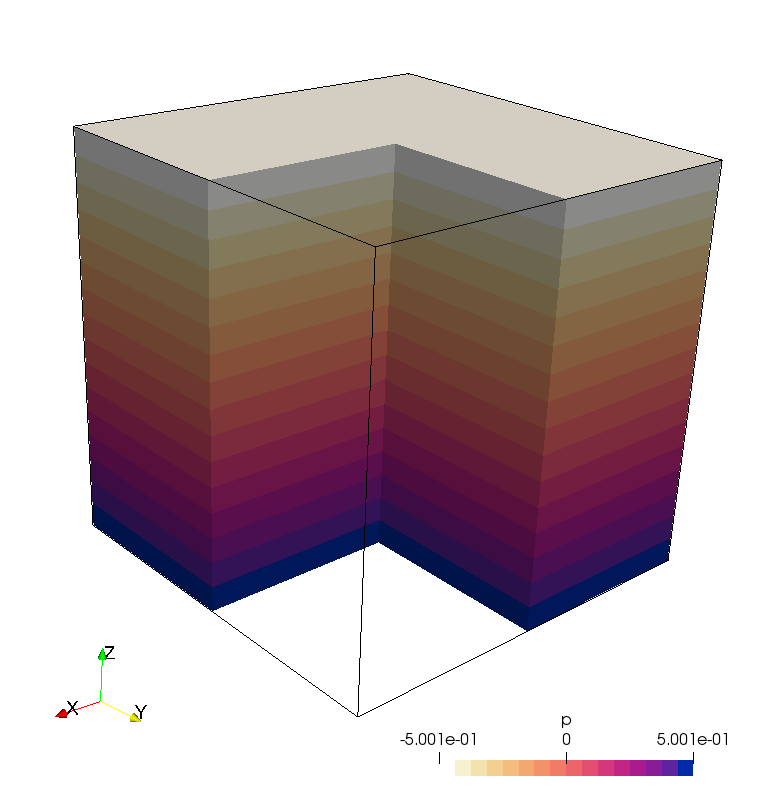
\includegraphics[width=6cm]{images/benchmark_annulus_mms/press}
\end{center}

This benchmark is of course very simple and the fact that the solution is independent of $\theta$
renders it not so useful. It has succesfully been implemented in \elefant.
